Historically, dxex is based on PythonPDEVS~\cite{PythonPDEVS}.
While Python is a good language to create software prototypes, its performance has proven to be insufficient to compete with other simulation kernels~\cite{MasterThesis}.
Dxex implements only a subset of PythonPDEVS, but makes some of its own additions.
The core simulation algorithm and optimizations, however, are highly similar.

While we will not make a detailed comparison with PythonPDEVS here, dxex also supports direct connection~\cite{SymbolicFlattening}, \textsf{Dynamic Structure DEVS}~\cite{DSDEVS}, termination conditions, and a modular tracing framework~\cite{PythonPDEVS}.
But whereas PythonPDEVS only supports optimistic synchronization, dxex support multiple synchronization protocols.
This is in line with the design principles of PythonPDEVS: offer users the option to pass information on how to efficiently simulate the model.
In our case, it now becomes possible to pass the simulation kernel the ``hint'' as to which synchronization protocol would be ideal for this model.
Furthermore, the implementation in C++11 allows many more (static) optimizations, which were plainly impossible when using an interpreted language.

Note that, since there is no universal \textsf{DEVS} model standard, dxex models are incompatible with PythonPDEVS and vice versa.
This is due to dxex models being grafted on C++11, whereas PythonPDEVS models are grafted on Python.

In the remainder of this section, we will elaborate on our prominent new feature: support for multiple synchronization protocols within the same simulation tool.

\subsection{Synchronization protocols}
We have previously shown that different synchronization protocols exist, with each of them being optimized for a specific kind of model.
As no single synchronization protocol is ideal, a general purpose simulation tool should support multiple situations.
Currently, however, most parallel simulation tools chose only a single synchronization protocol due to the inherent differences between these approaches.
An uninformed choice on which to implement is insufficient, as performance is likely to be bad.
We therefore argue that a real general purpose simulation tool should support sequential, conservative, and optimistic synchronization.

Each of them is applicable in specific model configurations.
Conservative synchronization is ideal when high lookahead exists between different nodes, and barely any blocking is necessary.
Optimistic synchronization is ideal when lookahead is unpredictable, or there are rare (almost) instantaneous events.
Finally, sequential simulation is still required for models where parallelism is bad, causing significant overhead.

\subsubsection{Sequential}
Our sequential simulation algorithm is very similar to the one found in PythonPDEVS, including most of its optimizations.
However, the simulation algorithm is designed to be overloaded by different synchronization protocol implementations.
This way, the \textsf{DEVS} simulation algorithm is implemented once, but parts can be overwritten as needed.
In theory, more synchronization protocols (\textit{e.g.}, other algorithms for conservative synchronization) can be added without altering our design.

An overview of this design is given in Figure~\ref{fig:class_diagram}.
It shows that there is a simulation \texttt{Core}, which has several \texttt{AtomicModels} connected to it.
The default \texttt{Core} is merely the sequential simulation core.
Its subclasses define specific variants of the simulation algorithm, like \texttt{ConservativeCore} (conservative synchronization), \texttt{OptimisticCore} (optimistic synchronization), and \texttt{DynamicCore} (\textsf{Dynamic Structure DEVS}).

\begin{figure}
    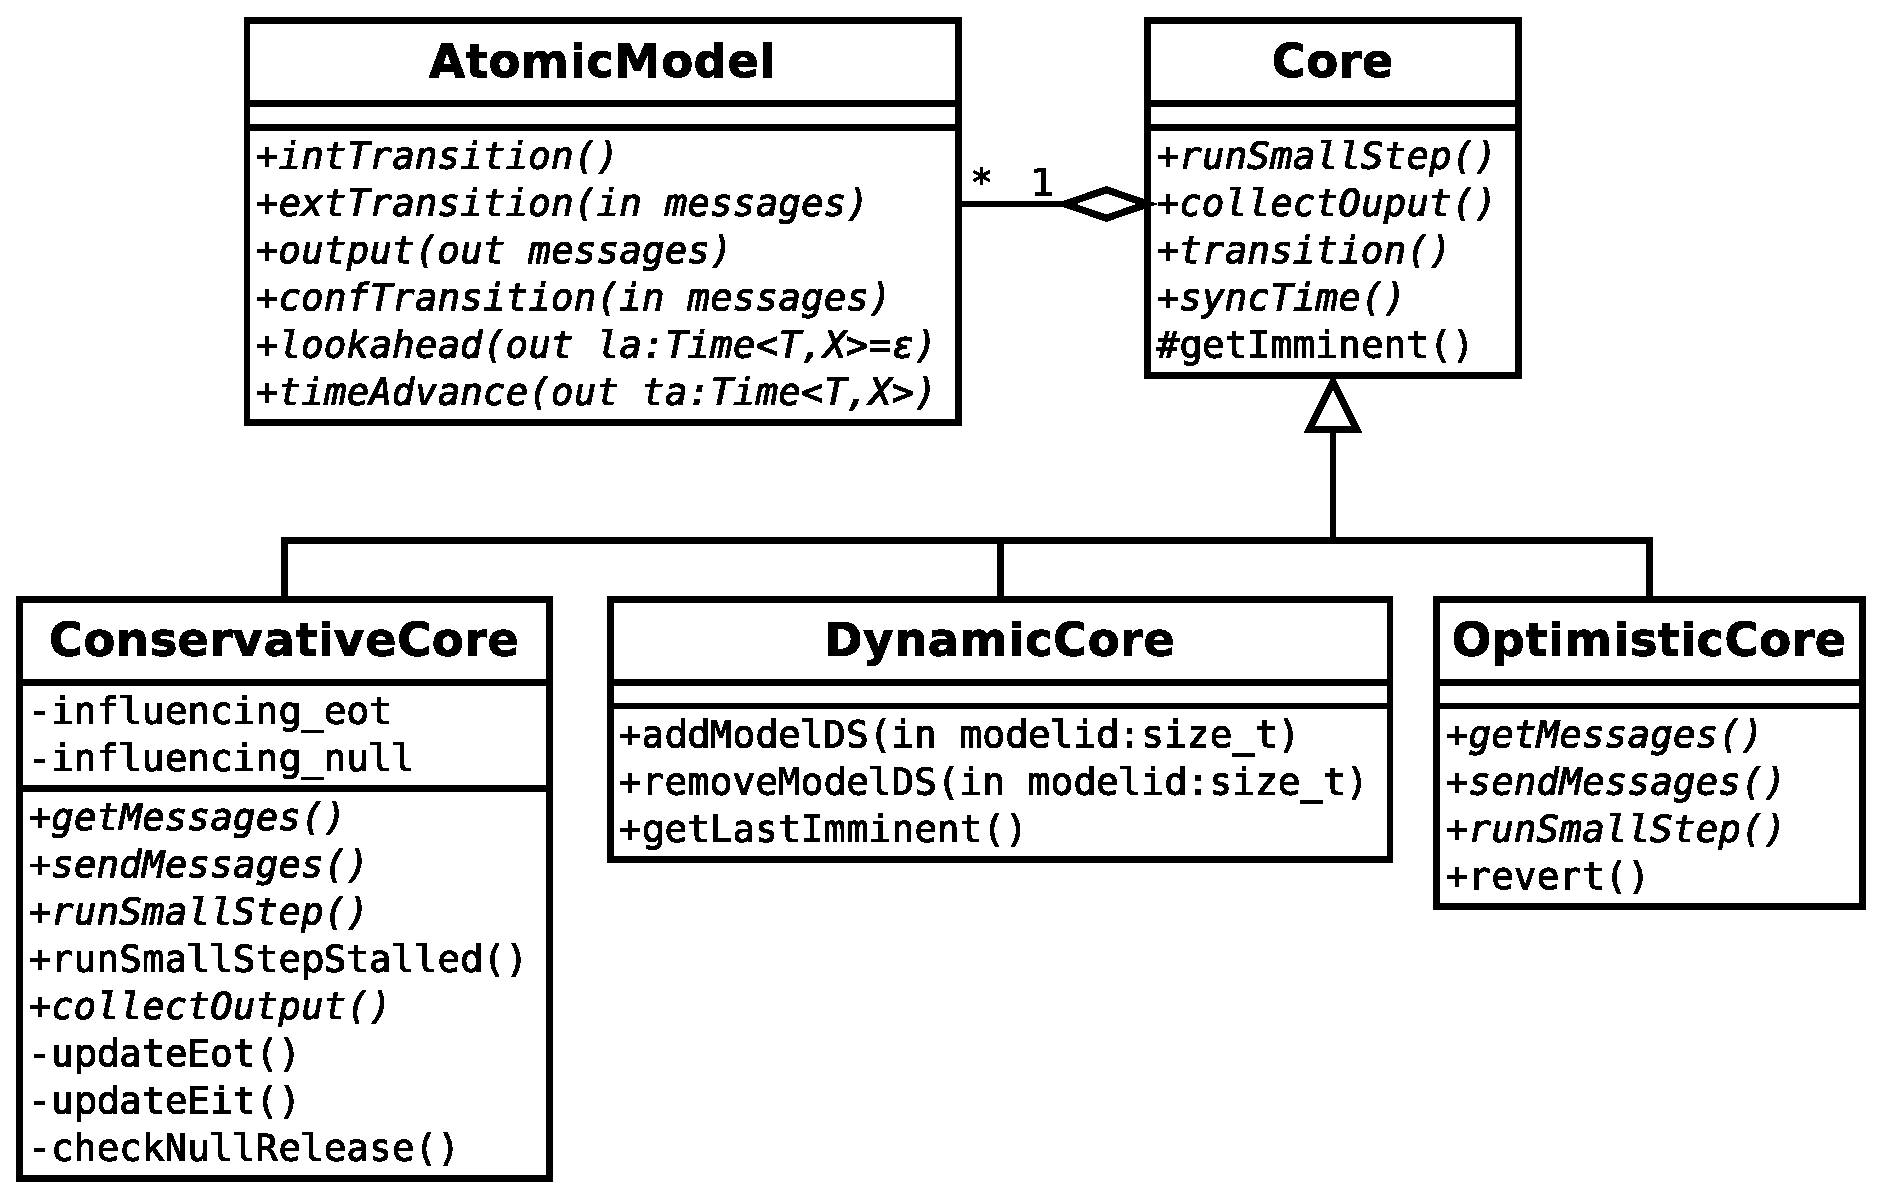
\includegraphics[width=\columnwidth]{fig/cores_class_diagram.eps}
	\caption{Dxex kernel design.}
	\label{fig:class_diagram}
\end{figure}

\subsubsection{Conservative}
For conservative synchronization, each node determines the nodes it is influenced by.
Each model provides a lookahead function, which determines the lookahead depending on the current simulation state.
Within this time interval, it is an error if a model raises an event, thus violating its previous promise.
The node uses this information to compute its earliest output time (EOT), and writes out the value in shared memory through the use of C++11 synchronization primitives.

\subsubsection{Optimistic}
For optimistic synchronization, each node needs to keep track of all intermediate simulation states.
This needs to be done carefully, in order to avoid unnecessary copies, and minimize the overhead induced for each transition function.
We use Mattern's GVT algorithm~\cite{mattern} to determine the Global Virtual Time (GVT) using at most $2n$ synchronization messages.
This process runs asynchronously from the simulation itself.
Once the GVT is found, all nodes are informed of the new value, after which fossil collection is performed.

\subsection{Transparancy}
A user must only provide one model, implemented in C++11, which can be simulated by each synchronization kernel.
The exception is conservative synchronization: a lookahead function is required, whereas this is not possible in other synchronization kernels.
Two options are possible: either a lookahead function is always provided, even when it is not required and possibly not used, or using a default lookahead function if none is defined.

Always defining a lookahead function might seem redundant, especially if users will never use conservative synchronization.
The more attractive option is for the simulation tool to provide a default lookahead function, defined by the minimum detected time advance.
This lookahead value is most likely too small, but will prevent causality errors at the cost of performance.
Depending on the model, simulation performance might still be faster than sequential simulation.

Defining a lookahead function is therefore recommended in combination with conservative synchronization, but is not a necessity.
